\documentclass[10pt,a4paper,oneside,fleqn]{report}
\usepackage{geometry}
\geometry{a4paper,left=20mm,right=20mm,top=1cm,bottom=2cm}
\usepackage[utf8]{inputenc}
%\usepackage{ngerman}
\usepackage{amsmath}                % brauche ich um dir Formel zu umrahmen.
\usepackage{amsfonts}                % brauche ich für die Mengensymbole
\usepackage{graphicx}
\setlength{\parindent}{0px}
\setlength{\mathindent}{10mm}
\usepackage{bbold}                    %brauche ich für die doppel Zahlen Darstellung (Einheitsmatrix z.B)
\usepackage[linktocpage={false}]{hyperref}


\usepackage{color}
\usepackage{titlesec} %sudo apt-get install texlive-latex-extra

\definecolor{darkblue}{rgb}{0.1,0.1,0.55}
\definecolor{darkred}{rgb}{0.55,0.2,0.2}

\titleformat{\chapter}[display]{\color{darkred}\normalfont\huge\bfseries}{\chaptertitlename\
\thechapter}{20pt}{\Huge}

\titleformat{\section}{\color{darkblue}\normalfont\Large\bfseries}{\thesection}{1em}{}
\titleformat{\subsection}{\color{darkblue}\normalfont\Large\bfseries}{\thesection}{1em}{}

% Notiz Box
\usepackage{fancybox}
\newcommand{\notiz}[1]{\vspace{5mm}\ovalbox{\begin{minipage}{1\textwidth}#1\end{minipage}}\vspace{5mm}}

\usepackage{cancel}


%\includegraphics[width=0.75\textwidth]{thepic.png}

\begin{document}
%\tableofcontents
\setcounter{chapter}{8}
\chapter{Energiebänder}


Oder warum unterscheiden wir zwischen Halbleiter, Leiter und Isolatoren.

'gute' Leiter: \(\rho\approx 10^{-10}\Omega \cdot cm\)
'gute' Isolator:  \(\rho\approx 10^{22}\Omega \cdot cm\)

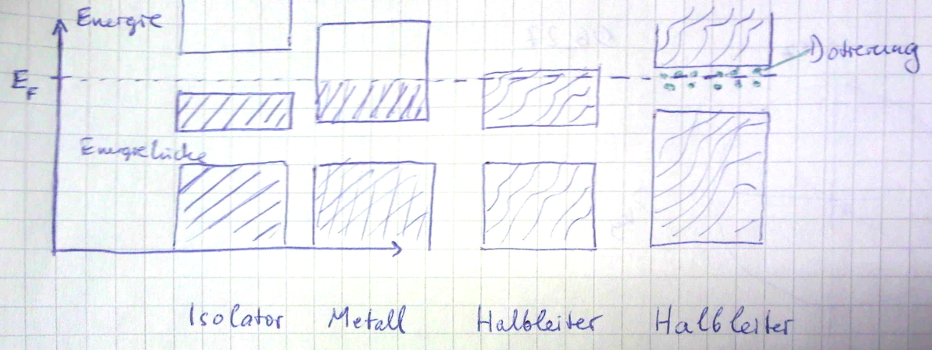
\includegraphics[width=0.75\textwidth]{kap06_31.png}

\underline{1 Beispiel}: Model des nahezu freien Elektronen

\(E_x=\frac{\hbar^2k^2}{2m}\); Wellenfunktion \(\psi_{\vec k} = e^{i\vec k\vec r}\)

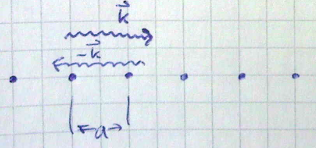
\includegraphics[width=0.75\textwidth]{kap06_32.png}

Laue (Bragg-Reflekton) \(-\vec k+\vec G = \vec k\) mit reziproken Gitter \(\vec G\)

\[ (-\vec k +\vec G)^2 = \vec k^2 \Rightarrow 2kG = G^2; \qquad k=\frac{G}{2}=\pm \frac{\pi}{2}n_G\]

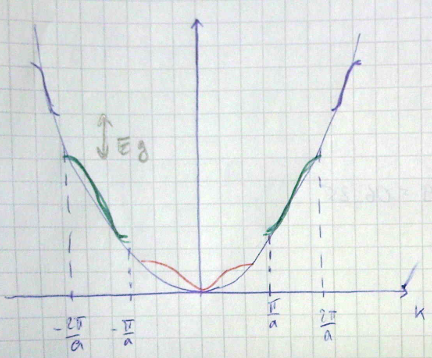
\includegraphics[width=0.75\textwidth]{kap06_33.png}

Zwei verschiedene Stehende Wellen:

\[ \psi_+ \propto e^{i\frac{\pi x}{a}}+e^{-i\frac{\pi x}{a}}=2cos\frac{\pi x}{a} \]
\[ \psi_- \propto e^{i\frac{\pi x}{a}}-e^{-i\frac{\pi x}{a}}=2isin\frac{\pi x}{a} \]

Gruppengeschwindigkeit \(v_G = \frac{\partial E_k}{\partial p} = \left.\frac{\hbar k}{m}\right|_{k=\pm\frac{\pi}{a}}=^!0;\)

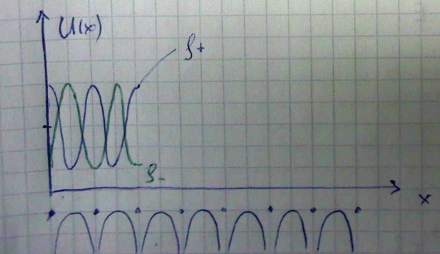
\includegraphics[width=0.75\textwidth]{kap06_34.png}

\[\rho_+=|\psi_+|^2 \propto cos^2\frac{\pi x}{a} = \frac{1}{2}(1+cos^2\frac{2\pi x}{a})\]
\[\rho_-=|\psi_-|^2 \propto sin^2\frac{\pi x}{a} = \frac{1}{2}(1-cos^2\frac{2\pi x}{a})\]


Wahrscheinlichkeitsdichte \(\psi^*\psi=|\psi|^2\); \(\rho_0=1e=e^{-ikx}e^{ikx}e\)

Erwartungswert der Potentiellen Energie: \(E_{\rho_+}<E_{\text{frei}}<E_{\rho_-}\), \(U(x)=U cos\frac{2\pi x}{4}\); 

\begin{align}
E_g &= \frac{1}{a}\int dx U(x)[|\psi_-|^2-|\psi_+|^2]\\
&=\frac{2U}{a}\int_0^a dx cos\frac{2\pi x}{4}\frac{1}{2}[1-cos\frac{2\pi x}{a}-1-cos\frac{2\pi x}{a}]\\
&= \frac{2U}{a}\int_0^a dx cos^2\frac{2\pi x}{a}\\
&= \frac{U}{a}\int_0^a dx (1+cos\frac{4\pi x}{a})\\
&=\frac{U}{a}\left.(x+\frac{a}{4\pi}sin\frac{4\pi x}{a})\right|_0^a \\
&\equiv U = E_B-E_A
\end{align}


Elektronen in einem periodischen Potential (QM)
\[ H\psi(\vec r) = [-\frac{\hbar^2}{2m}\nabla+\tilde V(\vec r) ]\psi (\vec r) = E\psi(\vec r) \]

Translationsinvariant: \(\tilde V(\vec r) = \tilde V(\vec r+\vec l)\)

Entwicklung nach reziproken Gittervektoren \(\vec G\) (blochscher Ansatz)

\[\tilde V(\vec r) = \sum_G\tilde V_G\cdot e^{i\vec G\vec r}\]
\[\psi(\vec r) = \sum_{k}c_ke^{ikr}\]
Einsetzen in die SGL:

\[\sum_{\vec k}\frac{\hbar^2 k^2}{2m}c_ke^{i\vec k\vec r}+\sum_{k',\vec G}c_{k'}\tilde V_G e^{i(k'+G)\vec r}\equiv \sum_kc_ke^{i\vec k\vec r}\]
Umbenennung (summe über alle \(k'\)): \(k'+\vec G = k \rightarrow \)

\[0=\sum_{\vec k}e^{i\vec k\vec r}\underbrace{\left[(\frac{\hbar^2 k^2}{2m}-E)c_k+\sum_G\tilde V_G c_{\vec k-\vec G}\right]}_{=0}\]


\[(\frac{\hbar^2 k^2}{2m}-E)c_k+\sum_G\tilde V_G c_{\vec k-\vec G}=0\]

Dieser Satz algebraischer Gleichungen ist die Darstellung der Schrödigner Gleichung im \(\vec k\)-Raum \(\Rightarrow\) \(E_k\)-Energie Eigenwert.

\begin{align}
\psi_k(\vec r) &= \sum_{\vec G}c_{\vec k-\vec G}e^{i(\vec k-\vec G)\vec r}\\
&= \underbrace{e^{i\vec k\vec r}}_{\text{ebene Welle}}\underbrace{\sum_{\vec G}c_{\vec k-\vec G}e^{-i\vec G\vec r}}_{U_k(\vec r)}\\
&= U_k(\vec r)e^{i\vec k\vec r}
\end{align}

Bloch Theorem: Die Eigenfunktionen der SG. für ein periodisches Potential sind das Produkt aus einer ebenen Welle und einer Funktion \(U_k(\vec r)\) mit der Periodizität des Gitters. 


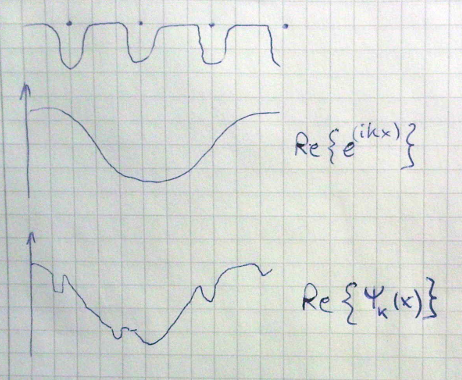
\includegraphics[width=0.75\textwidth]{kap06_35.png}
 
\begin{align}
\psi_k(\vec r+\vec R) &= \underbrace{U_k(\vec r+\vec R)e^{i\vec k\vec r}}_{\psi_{\vec r}}e^{i\vec k\vec R}
\end{align}

\[\psi_{k+G}(\vec r) \sum_G c_{k+g'-G}e^{i(\vec k+G'-G)\vec r}\]

Umbenennung \(G''=G-G'\)

\[\Rightarrow e^{i\vec k\vec r}\sum_{G''} \underbrace{c_{\vec k-\vec G''}e^{-i\vec G''\vec r}}_{U_{\vec k}(\vec r)}\]
\[\Rightarrow \psi_{\vec k+\vec a}(\vec r) = \psi_k(\vec r)\]

\[H\psi_{k+G}(\vec r) = E_{\vec k+\vec G'}\psi_{\vec k+\vec G'}(\vec r)\]
\[H\psi_{k}(\vec r) = E_{\vec k+\vec G'}\psi_{\vec k}(\vec r)\]
\[\Rightarrow E_{k+G'}=E_k\]

Lösung der SG. an der Grenze der Brillouin Zone. 

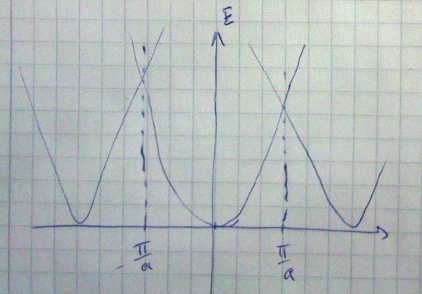
\includegraphics[width=0.75\textwidth]{kap06_36.png}

\[(E-\frac{\hbar^2}{2m}|k-G|^2 )c_{k-G}=\sum_G \tilde V_{G'}c_{k-G-G'}\]

\begin{align}
c_{k-G} &= \frac{\sum_G \tilde V_{G'}c_{k-G-G'}}{E-\frac{\hbar^2}{2m}|k-G|^2}\\
&= \frac{\sum_{G''}V_{G''-G}c_{k-G''}}{\frac{\hbar^2}{2m}(k^2-|k-G|^2)}
\end{align}

Umbenennung: \(G=G''-G\)
Nullstellen: \(k^2=|\vec k-\vec G|^2\)
Abkürzungen \(g=\frac{2\pi}{a}\); \(G=0\),\(G=g\); \(\lambda_k = \frac{\hbar^2 k^2}{2m}\)


Zwei Komponenten Näherung 

Erste Bedingung: \(\rightarrow (\lambda_k -E)c_k+\tilde V_g c_{k-g} = 0\)
zweite Bedingunge: \(\rightarrow (\lambda_{k-g} -E)c_{k-g}+\tilde V_g c_k = 0\)

Daraus resultieren Energieeigenwerte: \(E_{\pm}=\frac{1}{2}(\lambda_{k-g}+\lambda_k\pm \sqrt{(\lambda_{k-g}-\lambda_k)^2+\tilde V_g^2}\) und \(k=\frac{g}{2}\rightarrow \lambda_{k-g}=\lambda_k\)

An der Grenze der Brillouin Zone

\[ E_{\pm} = E_{\frac{g}{2}}\pm|\tilde V_g| \]

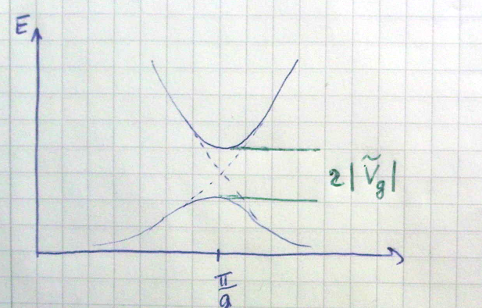
\includegraphics[width=0.75\textwidth]{kap06_37.png}

\(\frac{c_{k-G}}{c_k}=\frac{E-\lambda}{\tilde V_g}\)


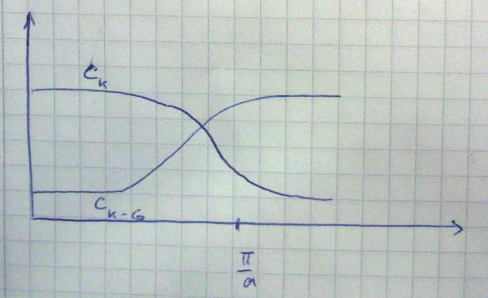
\includegraphics[width=0.75\textwidth]{kap06_38.png}



\section{Tight-binding Model}

\underline{'stark gebundene Elektronen'}


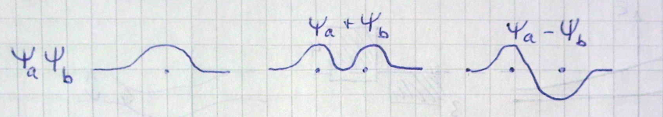
\includegraphics[width=0.75\textwidth]{kap06_39.png}

\[\rho \propto |\psi_a-\psi_b|^2\]


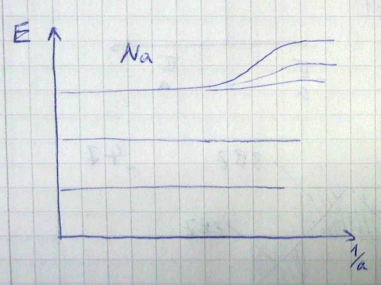
\includegraphics[width=0.75\textwidth]{kap06_40.png}
LCAO = Linear Combination of Atomic Orbitals

\[H\phi = E\phi\]
\[H= H_A+H_S\quad (m\neq n)\]
\[H = -\frac{\hbar^2}{2m}\nabla + \tilde V(\vec r - \vec R_m)\qquad R_m\equiv\text{Gittervektor}\]
\[H_S = \sum_{n\neq m}\tilde V_A(\vec r - \vec R_n)\]

Energie eigenwerte \(E_k\)

\[ E_k = \frac{\int \psi^* H\psi dV}{\int \psi^*\psi dV}\]

 \[\psi_{\vec k} = \sum_m a_m\phi(\vec r\cdot\vec R_m)\qquad a_m=\frac{1}{\sqrt{N}} e^{i\vec k\vec R_m}\quad N\equiv\text{Anzahl der Atome}\]


Bloch-Funktionen \(\rightarrow \) orthonormal Basis lokalisierter Zustände Wnnier-Funkitonen

\[w_m(\vec r\cdot\vec R_m) = \frac{1}{\sqrt{N}}\sum_{\vec k}e^{-i\vec k\vec R_m}\psi_k(\vec r- \vec R_m)\]
\[\psi =\frac{1}{\sqrt{N}}\sum_{\vec R_m}e^{i\vec k\vec R_m}w_m(\vec r- \vec R_m) \]
\[E_{\vec k} = \frac{1}{\underbrace{\int \phi^*\phi dV}_{=1\quad\text{Wellenfkt kaum Überlappung}}}\frac{1}{N}\sum_{m,n}e^{ik(Rm-R_n)}\int\phi^*(r-R_n)[H_A+H_S(\vec r-\vec R_m)\phi(\vec r-\vec R_m)dV]\]
\[\alpha = -\int \phi^*(r-R_m)H_s(\vec r-\vec R_m)\phi(\vec r -\vec R_m)dV \equiv\text{Energieänderung durch das Nachbarpotential}\]

\[\beta = -\int \phi^*(\vec r- \vec R_n)H_S(\vec r-\vec R_m)\phi(\vec r-\vec R_n)\equiv\text{Energieänderung durch den Überlapp der W.F.}\]

\begin{align}
E_{ki} &= E_i - \alpha_i - \sum\beta_{i,n}e^{ik(R_n-R_m}\\
&= E_i - \alpha_i2\beta_{i}(cos(k_xa)+cos(k_y a)
\end{align}

Für ein kubisch primitives Gitter \(R_m-R_n=(\pm a,00),(0\pm a,0),(0,a\pm a)\); \(\Rightarrow \) Entwickeln für kleine \(k\):

\[E_{k,i}=E_i - \alpha_i-6\beta_i+\beta_i a^2k^2\]



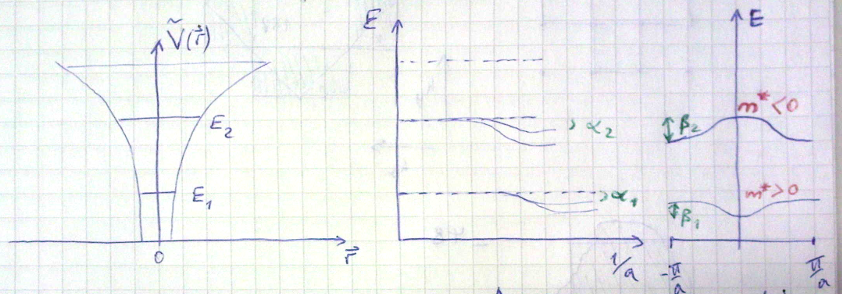
\includegraphics[width=0.75\textwidth]{kap06_41.png}

\[E_i=\frac{\hbar^2k^2}{2m}\Rightarrow m^*_i=\frac{\hbar^2}{2\beta_ia^2}\]

Energiedispersionspektrum \(E_i(k)\)

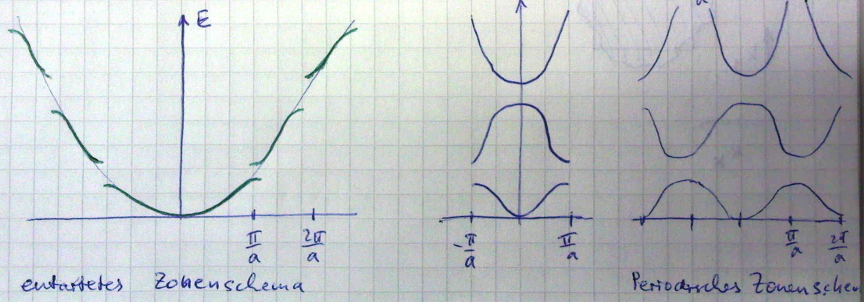
\includegraphics[width=0.75\textwidth]{kap06_42.png}


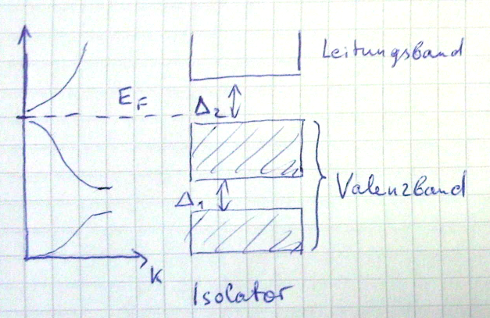
\includegraphics[width=0.75\textwidth]{kap06_43.png}

Isolator, \(\rho = 10^7-10^{14}\Omega m\); \(E_F = \frac{\hbar^2}{2m}(3\pi^2 n_e)^{2/3}\)

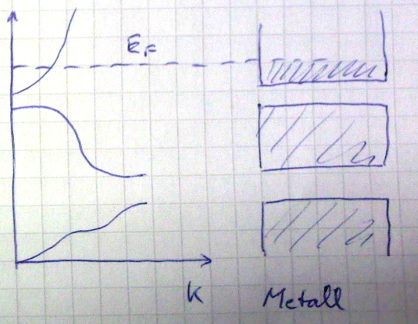
\includegraphics[width=0.75\textwidth]{kap06_44.png}

Metall: \(\rho = 10^{-4}-10^{-8}\Omega m\); 


2D-Gitter \(\rightarrow \) verschiedene Kristallrichtung


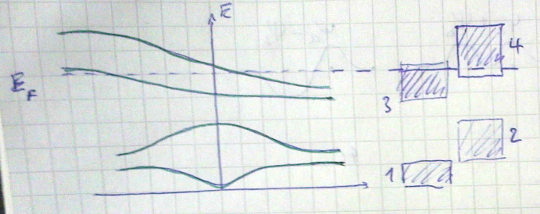
\includegraphics[width=0.75\textwidth]{kap06_45.png}


Halbmetalle As, Sb(Antimon), Bi 

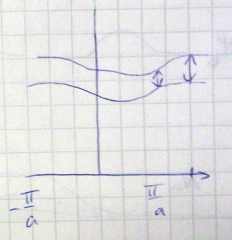
\includegraphics[width=0.75\textwidth]{kap06_46.png}




\section{Brillouin-Zonen und Fermi- Flächen}
Brillion-Zonen und Fermi Flächen (2D BZ)

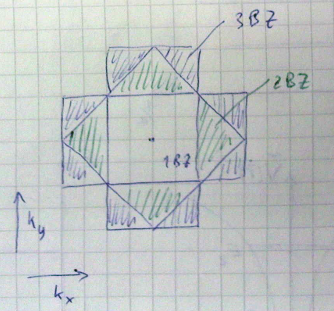
\includegraphics[width=0.75\textwidth]{kap06_47.png}

an der zonengrenze (stehende Wellen)
\[\frac{\partial\omega}{\partial k}=\frac{1}{\hbar}\vec \nabla E_\bot =0\]
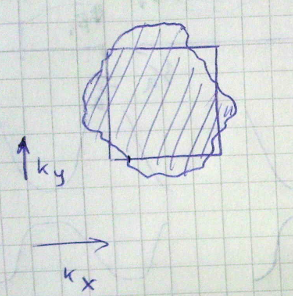
\includegraphics[width=0.75\textwidth]{kap06_48.png}






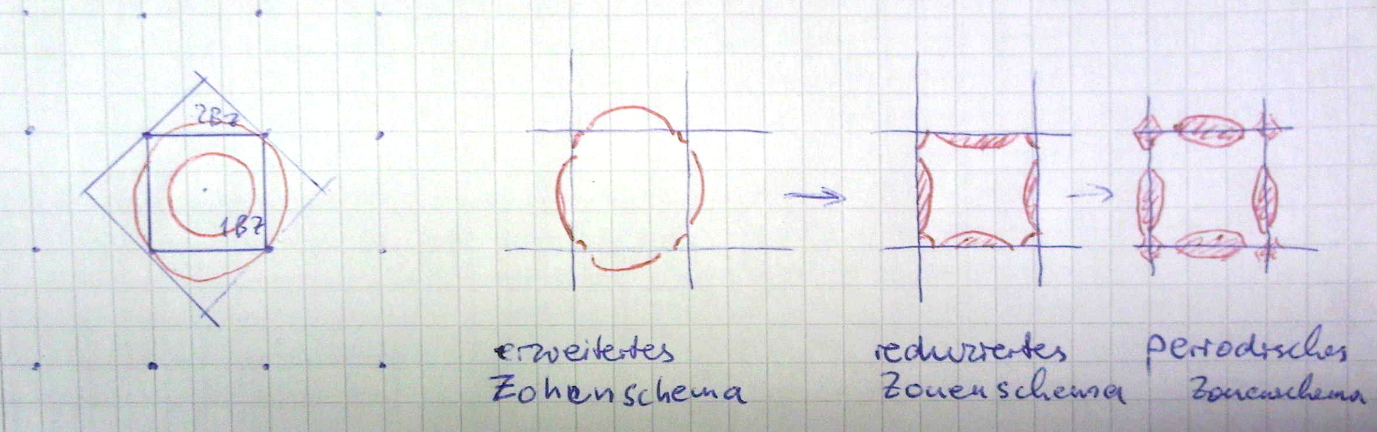
\includegraphics[width=0.75\textwidth]{kap06_49.png}




\end{document}
